\documentclass[contents.tex]{subfiles}

\begin{document}

\section{Summary}\label{sec:summary}
    This report was developed due to the curricular course RCOM(Computer Network) and it serves the purpose of concluding the first project of this course.
The project was finished successfully by implementing all the required functionalities, passing all the tests and building a fully working application while adding options that were not required specified further in the report.

% This section needs a lot of work.
\section{Introduction}
\label{sec:intro}

	This project’s goal is to transfer data from one computer to the other through a
	serial port using a protocol developed by us which includes reading, writing and data analysis functions. We did all this based on the script provided to us.
	In here you will be able to find all the functions used by us to achieve the goal
	and and explanation of almost everything using this structure:

Architecture - functional blocks and interfaces used
Code Structure - demonstration of the API’s, main data structuring, functions and how they relate to the architecture
Main use cases - sequence of functions with the help of diagrams created by us
Linking layer protocol - identification of the main functional aspects, description of those aspects implementation strategy with code samples
Application protocol - identification of the main functional aspects, description of those aspects implementation strategy with code samples
Validation - description of the tests used with data to back up the test results
LL protocol efficiency - stats that measure the protocol’s practical efficiency and also the theoretical efficiency used as comparison
Conclusion - reflection on the learning objectives achieved and also an overall view of the information detailed on the previous sections.

\subsection{Concepts}\label{sec:concepts}
\textbf{AL} - application Layer\\
\textbf{R} - receiver\\
\textbf{T} - transmitter\\
\textbf{LL} - link Layer\\
\section{Validation} \label{sec:validation}
	Some tests was implemented in order to prove the robustness of the program:
	\begin{description}
		\item[$\bullet$ a-] Send a file without errors
		\item[$\bullet$ b-] Force errors in the serial port with pins
		\item[$\bullet$ c-] Force errors in the program with specific functions with a specific probability to generate errors in data field and header field (introduceErrors())
		\item[$\bullet$ d-] Turn off the connection in the serial port and turn it on later
		\item[$\bullet$ e-] All the previous attempt of failures together.
\end{description}
	The program is robust to this errors and much probably others that we did not anticipate. After every single attempt to make the program fail, the connection continues and the file is sent perfectly.
	\begin{figure}%
		\centering
		\subfloat[]{{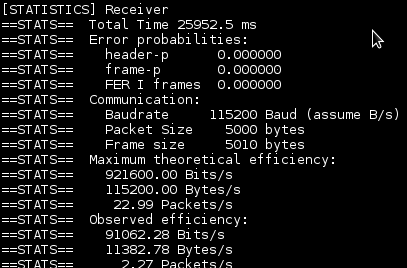
\includegraphics[scale=0.65]{p=0.png} }}\hfill
		\subfloat[]{{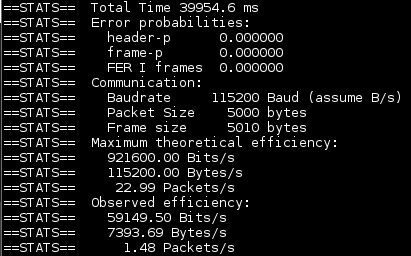
\includegraphics[scale=0.65]{bcc1-corrupted.png}}}\hfill
		\subfloat[]{{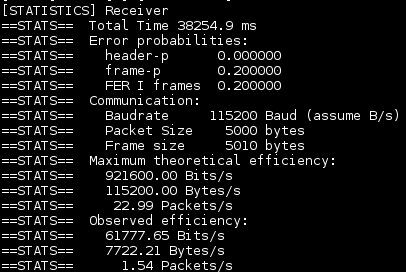
\includegraphics[scale=0.65]{p=20.png} }}\hfill
		\subfloat[]{{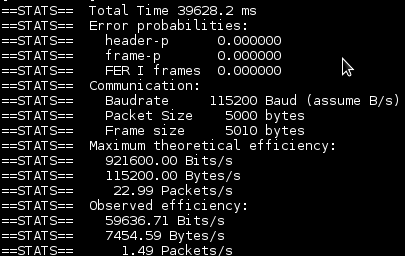
\includegraphics[scale=0.65]{cut-connection3times.png}}}\hfill
		\caption{Output stats for each case}%
		\label{fig:example}%
	\end{figure}

\section{Protocol Efficiency}\label{sec:pefficiency}
To approach this topic we analyze some charts. The first two charts use packets with 5000 bytes of data, baudrate = 115200 and the file has 295412 bytes which corresponds to 59 packets. 
\begin{figure}[!htb]
	\begin{minipage}{0.48\textwidth}
		\centering
		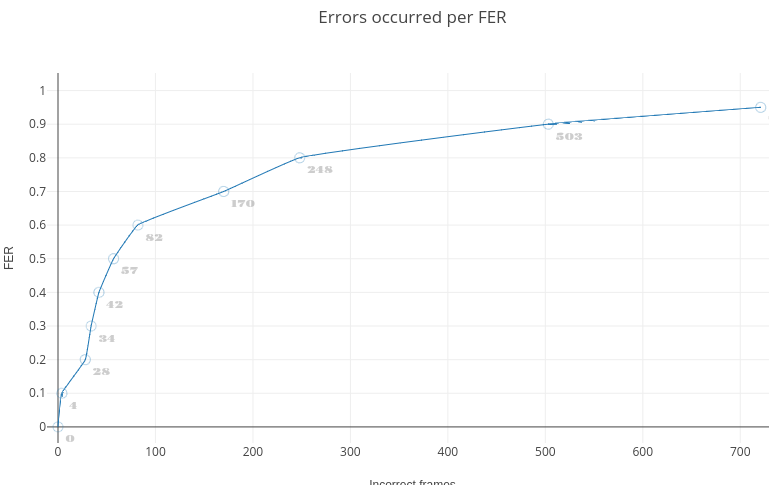
\includegraphics[scale=0.5]{graph1.png}
		\caption{Interpolation for Data 1}\label{Fig:Data1}
	\end{minipage}\hfill
	\begin{minipage}{0.48\textwidth}
		\centering
		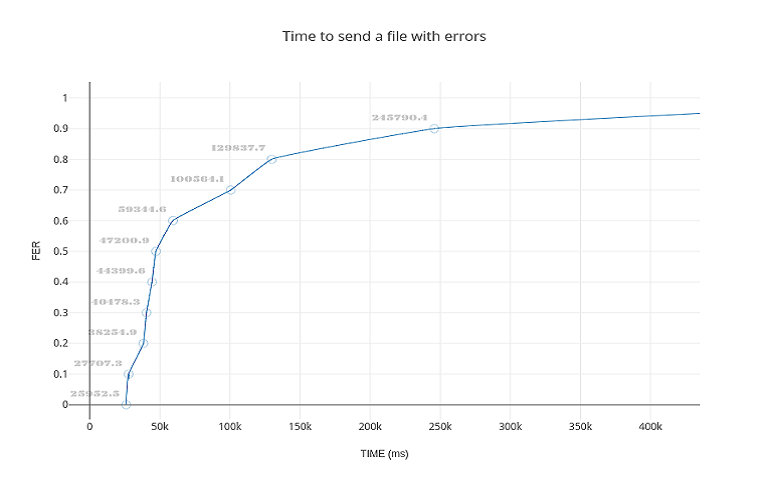
\includegraphics[scale=0.5]{graph2.png}
		\caption{Time to deliver a file with errors}\label{Fig:Data2}
	\end{minipage}
\end{figure}

\section{conclusion}\label{sec:conclusion}

We achieved all of the requirements specified on the script building a fully working project. We soaked in all of the concepts of the protocol and we wrote efficient code robust enough to work for multiple frames and to detect multiple failures.

The most challenging part in the development phase was building thellopen() and llclose() functions robust enough so that it detected many errors in the frames headers.

\end{document}
